\documentclass[aspectratio=169,xcolor=dvipsnames]{beamer}
% 1. Definir el color ANTES de llamar al tema SimplePlus
\usepackage{xcolor}
\definecolor{nyugray}{RGB}{128,128,128}
\usetheme{SimplePlus}
\definecolor{UnalGreen}{RGB}{0,153,51}
\usepackage[utf8]{inputenc}
\usepackage[spanish]{babel}
\usepackage{hyperref}
\usepackage{graphicx}
\usepackage{booktabs}
\usepackage{tikz}
\usepackage{pgfplots}
% NOTA: no se declara \pgfplotsset{compat=...} a propósito (ver convenciones del curso)
\usetikzlibrary{positioning, arrows.meta, babel}
\usepackage[skip=5pt]{caption}
\captionsetup{justification=justified, font=small}
\usefonttheme{professionalfonts}

% ----- PLACEHOLDER PARA IMÁGENES EXTERNAS -----
\newcommand{\imgwarning}[2][0.8]{%
	\begin{center}
		\fcolorbox{nyugray}{gray!8}{%
			\parbox[c][3.2cm][c]{#1\textwidth}{\centering\small\textcolor{nyugray}{%
					[\,Insertar imagen: #2\,]}}%
		}
	\end{center}
}

\title{Laboratorio Mecánica y ondas para Biociencias}
\subtitle{Sesión 2: Propagación de errores y Graficación}
\titlegraphic{%
	\vspace*{-0.3cm}%
	\IfFileExists{imagenes/universidad-nacional-de-colombia-sede-bogota-seeklogo.png}{%
		\includegraphics[width=2.2cm]{imagenes/universidad-nacional-de-colombia-sede-bogota-seeklogo.png}%
	}{%
		\IfFileExists{universidad-nacional-de-colombia-sede-bogota-seeklogo.png}{%
			
\includegraphics[width=2.2cm]{universidad-nacional-de-colombia-sede-bogota-seeklogo.png}%
		}{}%
	}%
	\hspace{1.0cm}%
	\IfFileExists{logoMIAI_white.png}{%
		
\includegraphics[width=4.0cm]{logoMIAI_white.png}%
	}{%
		\IfFileExists{imagenes/logoMIAI_white.png}{%
			\includegraphics[width=4.0cm]{imagenes/logoMIAI_white.png}%
		}{}%
	}%
}
\author{Miguel Andrés Perdomo Gutiérrez}
\institute{%
	Auxiliar Docente | M.Sc. en Ciencias -- Física\\
	Universidad Nacional de Colombia -- Sede Bogotá
}
\date{11 de septiembre de 2026}

\begin{document}
	
	% ============================================================
	% SLIDE 1: PORTADA
	% ============================================================
	\begin{frame}
		\titlepage
	\end{frame}
	
	% ============================================================
	% SLIDE 2: AGENDA DE LA SESIÓN
	% ============================================================
	\begin{frame}{Agenda de la Sesión}
		\centering
		\begin{tikzpicture}[
			box/.style={rectangle, rounded corners, draw=UnalGreen, thick, fill=UnalGreen!10,
				minimum width=2.4cm, minimum height=1.7cm, align=center, font=\small},
			arr/.style={-{Latex[length=2mm]}, thick, UnalGreen}
			]
			\node[box] (b1) {Sustentación\\Taller 2\\\textbf{45 min}};
			\node[box, right=0.5cm of b1] (b2) {Grupos de\\trabajo\\\textbf{5 min}};
			\node[box, right=0.5cm of b2] (b3) {Cinemática 2D:\\Tiro parabólico\\\textbf{60 min}};
			\node[box, right=0.5cm of b3] (b4) {Preguntas\\y dudas\\\textbf{10 min}};
			\draw[arr] (b1) -- (b2);
			\draw[arr] (b2) -- (b3);
			\draw[arr] (b3) -- (b4);
		\end{tikzpicture}
		
		\vspace{0.5cm}
		\begin{itemize}
			\item Duración total: \textbf{2 horas} (Viernes 09:00--11:00, Edificio 401, Salón 202).
			\item Primera parte: sustentación en tablero del Taller 2 (Cinemática 1D y Graficación).
			\item Segunda parte: extensión a dos dimensiones -- movimiento de proyectiles.
		\end{itemize}
	\end{frame}


	% ============================================================
	% SLIDE 6: INCISO -- ¿QUÉ HACE BUENA UNA GRÁFICA?
	% =====================================
	
		% ============================================================
	% SLIDE 6: LOS DATOS
	% ============================================================
	\begin{frame}{Los datos: volumen de un gas vs.\ temperatura}
		\begin{center}
			\footnotesize
			\begin{tabular}{lccccccccc}
				\toprule
				$T$ ($^\circ$C) & 62.3 & 68.6 & 81.4 & 87.4 & 98.6 & 104.5 & 116.9 & 121.2 & 135.0 \\
				\midrule
				$V$ (cm$^3$) & 27073 & 28492 & 29300 & 29200 & 30849 & 31500 & 32100 & 32000 & 33500 \\
				\bottomrule
			\end{tabular}
		\end{center}
		
		\vspace{0.4cm}
		\begin{center}
			\small
			Los mismos datos se graficaron de tres maneras distintas.
			Observen cada panel y decidan cuál usarían en un informe y por qué.
		\end{center}
	\end{frame}
	
	% ============================================================
	% SLIDE 7: PANEL (a)
	% ============================================================
	\begin{frame}{Panel (a)}
		\begin{center}
			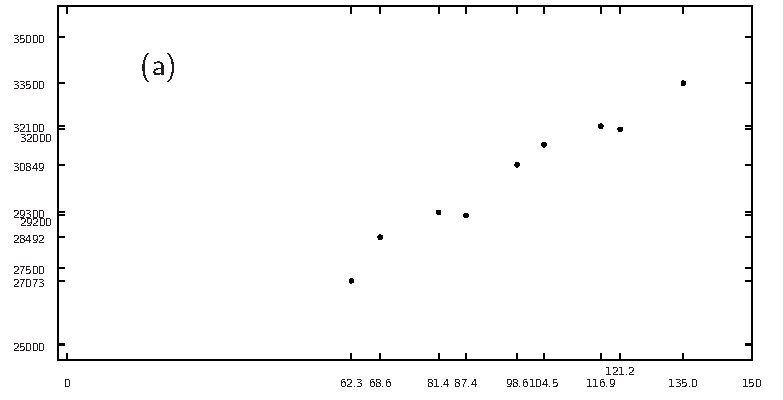
\includegraphics[width=\textwidth,height=0.85\textheight,keepaspectratio]{figura1.pdf}
		\end{center}
	\end{frame}
	
	% ============================================================
	% SLIDE 8: PANELES (b) Y (c)
	% ============================================================
	\begin{frame}{Paneles (b) y (c)}
		\begin{center}
			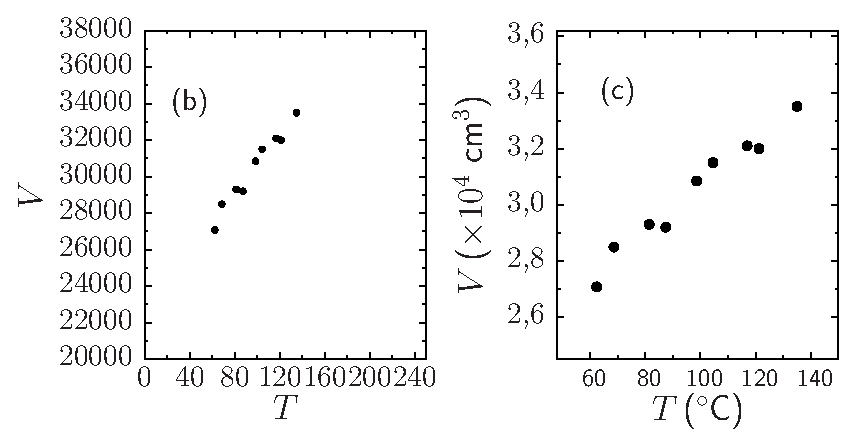
\includegraphics[width=\textwidth,height=0.85\textheight,keepaspectratio]{figura2.pdf}
		\end{center}
	\end{frame}
	% ============================================================
	% SLIDE 9: ¿CÓMO LES FUE CON LA GRAFICACIÓN?
	% ============================================================
	\begin{frame}{La parte opcional: midiendo $g$}
		\begin{columns}[T]
			\begin{column}{0.5\textwidth}
				\small
				La idea de Galileo: si
				\[
				h = \tfrac{1}{2}g\,t^2
				\]
				entonces al graficar $h$ contra $t^2$ (\textbf{no} contra $t$) se obtiene una \textbf{recta}
				de pendiente $m = g/2$.
				
				\vspace{0.25cm}
				\[
				g_{\text{exp}} = 2 \times m
				\]
				
				\vspace{0.25cm}
				\textcolor{UnalGreen}{\textbf{¿Quiénes lo intentaron?}}
				\begin{itemize}\small
					\item ¿Qué valor de $g$ obtuvieron?
					\item ¿Los puntos quedaron alineados?
				\end{itemize}
			\end{column}
			\begin{column}{0.5\textwidth}
				\begin{center}
					\begin{tikzpicture}
						\begin{axis}[width=6.0cm, height=4.6cm,
							xlabel={$t^2$ (s$^2$)}, ylabel={$h$ (m)},
							xmin=0, xmax=2.2, ymin=0, ymax=11,
							xtick={0,0.5,1,1.5,2}, ytick={0,2,4,6,8,10},
							grid=both, grid style={gray!30, thin}]
							\addplot[only marks, mark=*, mark size=1.8pt, UnalGreen]
							coordinates {(0.408,2) (0.816,4) (1.224,6) (1.633,8) (2.041,10)};
							\addplot[domain=0:2.2, samples=2, thick, red!70!black, dashed] {4.9*x};
						\end{axis}
					\end{tikzpicture}
				\end{center}
				\vspace{-0.2cm}
				\begin{center}
					\scriptsize Pendiente $m \approx 4.9 \Rightarrow g \approx 9.8$ m/s$^2$
				\end{center}
			\end{column}
		\end{columns}
	\end{frame}
	

	\begin{frame}{¿Preguntas o Comentarios?}
		\begin{center}
			\vspace{0.5cm}
			\Large Nos vemos la próxima sesión.
			
			\vspace{0.8cm}
			\normalsize
			mperdomog@unal.edu.co
			
			\vspace{0.2cm}
			Edificio 401 -- Salón 202
		\end{center}
	\end{frame}
	
\end{document}